% This is samplepaper.tex, a sample chapter demonstrating the
% LLNCS macro package for Springer Computer Science proceedings;
% Version 2.20 of 2017/10/04
%
\documentclass[runningheads]{llncs}
%
\usepackage{graphicx}
\usepackage{hyperref}
\usepackage{amsmath}

% Used for displaying a sample figure. If possible, figure files should
% be included in EPS format.
%
% If you use the hyperref package, please uncomment the following line
% to display URLs in blue roman font according to Springer's eBook style:
% \renewcommand\UrlFont{\color{blue}\rmfamily}

\usepackage[utf8x]{inputenc}
\usepackage[english,russian]{babel}


\begin{document}
%
\title{Acceleration of Global Search through Dual Lipschitz Constant Estimates
\thanks{This research was supported by the the Russian Science Foundation,
project No.\,16-11-10150.}}
%
\titlerunning{Acceleration of Global Search}
% If the paper title is too long for the running head, you can set
% an abbreviated paper title here
%
\author{Roman Strongin%\orcidID{0000-0003-0390-6695} 
\and Konstantin Barkalov%\orcidID{0000-0001-5273-2471} 
\and Semen Bevzuk%\orcidID{0000-0002-3845-5356}
}
%
\authorrunning{R. Strongin et al.}
% First names are abbreviated in the running head.
% If there are more than two authors, 'et al.' is used.
%
\institute{
Lobachevsky State University of Nizhni Novgorod, Nizhni Novgorod, Russia
\email{konstantin.barkalov@itmm.unn.ru}
}
%
\maketitle              % typeset the header of the contribution
%
\begin{abstract}
The paper considers global optimization problems with a black-box objective 
function satisfying the Lipschitz condition. Efficient algorithms for this 
class of problems require reliable estimates of the Lipschitz constant to be 
introduced. The various approaches have been proposed to take into account both
global and local properties of the objective function. In particular, algorithms
using local estimates of the Lipschitz constant have shown their potential.
The new approach presented in this paper is based on simultaneous use of two
estimates: one is substantially larger than the other. 
The larger estimate ensures global convergence and the smaller one reduces 
the total number of trials needed to find the global optimizer.
Results of numerical experiments on the random sample of multidimensional 
functions demonstrate the efficiency of the suggested approach.  

\keywords{Global optimization \and Multiextremal problems 
\and Lipschitz constant estimates}
\end{abstract}
%
%
%
\section{Introduction}

The paper considers global optimization problems of the form 
\begin{gather}
 \varphi(y^\ast)=\min{\left\{\varphi(y):y\in D\right\}}, \label{problem}\\
 D=\left\{y\in R^N: a_i\leq y_i \leq b_i, 1\leq i \leq N\right\} \label{D},
\end{gather}
where the objective function is a black-box function and assumed to satisfy the Lipschitz condition
\[
\left|\varphi(y_1)-\varphi(y_2)\right|\leq L\left\|y_1-y_2\right\|,\; y_1,y_2 \in D,
\]
with the constant $L$ unknown a priori.

Предположение липшицевости целевой функции является типичным для многих подходов к разработке алгоритмов глобальной оптимизации \cite{Pinter1996,Strongin2000,Zilinskas2010,Evtushenko2013}. При этом наиболее важной проблемой, так или иначе решаемой в данных алгоритмах, является адаптивная оценка неизвестной константы Липшица на основе полученной поисковой информации. 

Значение константы Липшица существенно влияет на скорость сходимости алгоритмов липшицевой глобальной оптимизации, поэтому столь важным является вопрос ее корректной оценки. Заниженная оценка инстинного значения константы Липшица может привести к потере сходимости алгоритма к глобальному решению. В то же время слишком большое значение оценки константы $L$ для целевой функции, %предполагает сложную структуру функции с резкими перепадами ее значений. Поэтому завышенная оценка константы L, 
не соответствующее ее истинному поведению, влечет за собой медленную сходимость алгоритма к точке глобального минимума. 

Известны несколько типичных способов адаптивного оценивания константы Липшица:
\begin{itemize}
	\item глобальная оценка константы Липшица $L$ во всей области поиска $D$ \cite{Horst1996,Pinter1996,Strongin2000}.
	\item локальные оценки константы Липшица $L_i$ в различных подобластях $D_i$ области поиска $D$ \cite{Kvasov2003,Sergeyev2010,Sergeyev2016}.
	\item выбор оценок константы $L$ из некоторого множества возможных значений \cite{Jones1993,Gablonsky2001,Jones2009,Sergeyev2006}.
\end{itemize}

Каждый из указанных подходов обладает своими достоинствами и недостатками. Например, использование только глобальной оценки во всей области поиска может замедлить сходимость алгоритма к точке глобального минимума. А использование локальных оценок, ускоряющих сходимость, требует адекватной настройки параметров алгоритма для сохранения глобальной сходимости. 

В данной работе рассмотрен алгоритм, котором предлагается использовать две глобальных оценки константы Липшица, одна из которых значительно больше другой. 
The larger estimate ensures global convergence and the smaller one reduces the total number of trials needed to find the global optimizer.
Выбор того, какая из двух оценок будет использоваться в правилах алгоритма, осуществляется адаптивно, в зависимости от поведения функции и фазы поиска.

Строгое обоснование предложенного подхода выходит за рамки данной первоначальной публикации и будет сделано в последующих работах. Здесь же приведем результаты вычислительных экспериментов, наглядно демонстрирующие эффективность нового алгоритма. При проведении вычислительных экспериментов было решено несколько сотен тестовых многоэкстремальных задач разной размерности.


\section{Global search algorithm and dimensionality reduction}

Типичным способом конструирования алгоритмов глобальной оптимизации является адаптация эффективных алгоритмов для решения одномерных задач к решению многомерных задач, see, for example, the diagonal partitions method in \cite{Sergeyev2006} or the simplicial partitions method in \cite{Zilinskas2008}.

В данной статье используется подход, основанный на идеях редукции размерности с помощью Peano-Hilbert curves \cite{Strongin2000,Sergeyev2013}, which continuously and unambiguously maps the unit interval $[0,1]$ onto the $n$-dimensional cube $D$ from (\ref{D}). By using this kind of mapping it is possible to reduce the multidimensional problem (\ref{problem}) to a univariate problem
\[
\varphi(y^\ast)=\varphi(y(x^\ast))=\min{\left\{\varphi(y(x)): x\in[0,1]\right\}},
\]
where the function $\varphi(y(x))$ will satisfy a uniform H{\"o}lder condition
\[
\left|\varphi(y(x_1))-\varphi(y(x_2))\right|\leq H\left|x_1-x_2\right|^{1/N},
\]
with the H{\"o}lder constant $H$ linked to the Lipschitz constant $L$ by the relation
$ H=2 L \sqrt{N+3}$.

Let us call the process of computing a function value (including the construction of the image $y=y(x)$) a \textit{trial}, and the pair $\{x, z = \varphi(y(x))\}$ the outcome of the trial.

The global search algorithm (according to \cite{Strongin2000}) can be formulated as follows.
The first two trials are executed at 
the points $y^0=y(0), y^1=y(1)$. The choice of the point $y^{k+1},k\geq 1,$  
for the next $(k+1)$-th trial is defined by the following rules.

\begin{enumerate}
	\item 
	Renumber the preimages of all the points $y^i=y(x^i)$
	from the trials already performed  	
%\begin{equation}\label{y_i} 
%y^0=y(x^0), y^1=y(x^1),...,y^k=y(x^k)
%\end{equation}
by subscripts in the increasing order of their coordinates, i.e.
\begin{equation}\label{x_i}
0=x_0<x_1<\dots <x_k=1,
\end{equation}
and associate these with the values $z_i=\varphi(y(x_i)), 0\leq i \leq k,$ 
computed at these points.
\item
Compute the maximum absolute value of the first divided differences
\begin{equation}\label{mu}
\mu = \max_{1 \leq i \leq k}\frac{\left|z_i-z_{i-1}\right|}{\Delta_i},
\end{equation}
where $\Delta_i=\left(x_i-x_{i-1}\right)^{1/N}$. If $\mu = 0$, set $\mu = 1$.
\item
For each interval $(x_{i-1}, x_i), \; 1\leq i \leq k,$  calculate the value 
$R(i)$ called the \textit{characteristic} of the interval
\begin{equation}\label{R}
R(i)=\Delta_i+\frac{(z_i-z_{i-1})^2}{r^2\mu^2\Delta_i}-2\frac{z_i+z_{i-1}-2z^*}{r\mu},
\end{equation}
where 
\begin{equation}\label{z}
z^*= \min_{0\leq i\leq k}z_i
\end{equation} 
and the real number $r>1$ is 
the input parameter of the algorithm.
\item 
Select the interval $(x_{t-1},x_t)$ corresponding to the maximum characteristic
\begin{equation}\label{MaxR}
R(t)= \max_{1 \leq i \leq k}R(i).
\end{equation}
\item
Carry out the next trial at the point $x^{k+1}\in(x_{t-1},x_t)$ calculated using
the following formula
\begin{equation}\label{xk1}
x^{k+1} = \frac{x_t+x_{t-1}}{2} - \mathrm{sign}(z_t-z_{t-1})\frac{1}{2r}
\left[\frac{\left|z_t-z_{t-1}\right|}{\mu}\right]^N.
\end{equation}
\end{enumerate}

The algorithm terminates if the condition $\Delta_t < \epsilon$ is satisfied
where $t$ is from (\ref{MaxR}), and $\epsilon>0$ is the predefined accuracy. 

The theory of convergence of this algorithm is provided in \cite{Strongin2000}.
%The modifications taking into account .... are given in [....].

\section{Algorithm with Dual Lipschitz Constant Estimates}

Алгоритм глобального поиска, изложенной в предыдущем разделе, предназначен для решения многоэкстремальных задач, в которых целевая функция удовлетворяет условию Липшица. При этом для для работы алгоритма не требуется задания  значений константы. Оценка константы осуществляется в процессе глобального поиска на основе имеющейся поисковой информации. 
В соответствии с теоремой \cite{Strongin2000}, последовательность точек испытаний $\{y^k\}$ будет сходиться к global minimizer $y^*$, если выполнено условие  
\begin{equation}\label{cond}
r\mu > 2^{3-1/N}L\sqrt{N+3}.
\end{equation}
Таким образом, подходящий выбор параметра $r$ из (\ref{R}) позволяет использовать значение $r\mu / 2^{3-1/N}\sqrt{N+3}$ как оценку константы Липшица для целевой функции $\varphi(y)$.

Выполнение условия (\ref{cond}) будет гарантировано при выборе большого значения параметра $r$, однако при этом метод выполнит большое количество испытаний до выполнения условия остановки.
Выбор малого значения параметра $r$ (что соответствует заниженной оценке константы Липшица) значительно сократит число испытаний, но может нарушить сходимость к глобальному экстремуму.

Перспективным является подход, при котором в правилах алгоритма будут использованы две оценки константы Липшица, одна из которых будет значительно выше другой, что соответствует использованию в алгоритме двух парметров $r_{glob}$ и $r_{loc}$, где $r_{glob} > r_{loc}$.

Правила алгоритма с двойной оценкой константы Липшица будут полностью повторять алгоритм глобального поиска, за исключением правила 3 (вычисление характеристики).

Новое правило вычисления характеристики $R(i)$ интервала $(x_{i-1}, x_i)$ будет состоять из следующих действий:
\begin{itemize}
\item
Вычислить значение $R_{glob}(i)$, соответствующее большей оценке константы Липшица
\[
R_{glob}(i)=\Delta_i+\frac{(z_i-z_{i-1})^2}{r_{glob}^2\mu^2\Delta_i}-2\frac{z_i+z_{i-1}-2z^*}{r_{glob}\mu}.
\]
\item
Вычислить значение $R_{loc}(i)$, соответствующее меньшей оценке константы Липшица
\[
R_{loc}(i)=\Delta_i+\frac{(z_i-z_{i-1})^2}{r_{loc}^2\mu^2\Delta_i}-2\frac{z_i+z_{i-1}-2z^*}{r_{loc}\mu}.
\]
\item
Определить характеристику интервала $R(i)$ как
\begin{equation}\label{pho}
R(i) = \max\{\rho R_{loc}(i),R_{glob}(i)\}, где \rho = \left(\frac{1-1/r_{glob}}{1-1/r_{loc}}\right)^2,
\end{equation}
и зафиксировать значение $r = r_{loc}$, если  $\rho R_{loc}(i) > R_{glob}(i)$, иначе зафиксировать $r=r_{glob}$.
Данное значение $r$ будет использовано в правиле 5 алгоритма при вычислении точки нового испытания.   
\end{itemize}.

Указанный способ вычисления характеристики имеет следующее обоснование. 
Пусть текущее минимальное значение $z^*$ из (\ref{z}) достигается в левой точке $i$-го интервала, т.е. $z^* = z_{i-1}$. Тогда, в соответствии с правилом (\ref{R}), будут верно неравенство
\[
R(i) \geq \Delta_i \left( 1 - \frac{1}{r} \right)^2.
\]
Следовательно, две нижние оценки для двух характеристик текущего лучшего интервала $R_{loc}(i)$ и $R_{glob}(i)$, вычисленных с разными параметрами $r_{loc}$ и $r_{glob}$, будут иметь разные значения.
Однако если первую из них домножить на коэффициент $\rho$ из (\ref{pho}), то нижние оценки характеристик лучшего интервала будут совпадать, что сделает сравнимыми и характеристики, вычисленные для остальных интервалов.

\section{Numerical Experiments}

The numerical comparison of the algorithms has been carried out using the GKLS 
test problem generator \cite{Gaviano2003}. 
This generator of multiextremal functions is often used for the investigations of the global 
optimization algorithms ~\cite{Paulavicius2014,Sergeyev2015,%Lebedev2015,Gergel2015,
Barkalov2018}.
%This generator allows multiextremal optimization problems to be generated with known properties (the number of localminima, the size of their domains of attraction, the global minimizer, etc.). 
Six GKLS classes of differentiable test functions of the dimensions $N = 3,4,5$
have been used. For each dimension, both \textit{Hard} and \textit{Simple}
classes have been considered. The difficulty of a class was increased either by
decreasing the radius of the attraction region of the global minimizer, or by
decreasing the distance from the global minimizer $y^\ast$ to the domain
boundaries. The global minimizer $y^\ast$ was considered to be found, if the
algorithm generated a trial point $y^k$ in the vicinity of the global minimum,
i.e. $\left|y^k-y^\ast\right| <\delta\left\|b-a\right\|$, where $\delta = 0.01$,
$a$ and $b$ are the boundaries of the search domain $D$. 

%УКАЗАТЬ ПРАВИЛЬНЫЕ ПАРАМЕТРЫ
When using the Global Search Algorithm, the parameter $r$ was set to $5$, 
the evolvent construction parameter was fixed as $m = 10$. 
The maximum allowable number of iterations per problem was $K_{max} = 10^6$.

Каждая серия задач была решена с помощью исходного алгоритма глобального поиска (GSA) и спомощью метода с двойной оценкой константы Липшица (GSA-DL). Среднее число итераций, выполненное алгоритмами, отражено в табл. \ref{tab:1}.
При этом при решении задач класса Simple в GSA использовалось единственное значение параметра $r=4.8$, при решении задач класса Hard -- $r=5.6$.
Указанное значение является минимальным (с точностью 0.1) значением, при котором успешно решились все задачи.
При решении данных классов задач с использованием GSA-DL указанное ранее значение параметра $r$ выбиралось для верхней оценки константы Липшица, т.е. задавалось значение $r_{glob} = r$, которое дополнялось значениями $r_{loc}=1.8$ и $r_{loc}=2.4$. 
%Структуру таблицы можно взять из статьи 

\begin{table}
	\caption{Average number of iterations}
	\label{tab:1}
	\center
	\begin{tabular}{ccccccccc}
		\hline\noalign{\smallskip}
		$r$ & \multicolumn{2}{c}{$N=3$} & & \multicolumn{2}{c}{$N=4$} & & \multicolumn{2}{c}{$N=5$}  \\
		\noalign{\smallskip} \cline{2-3} \cline{5-6} \cline{8-9} \noalign{\smallskip}
		 & \textit{Simple} & \textit{Hard} & & \textit{Simple} & \textit{Hard} & & \textit{Simple} & \textit{Hard}  \\
		\noalign{\smallskip} \hline \noalign{\smallskip}
									AGS	&	2502	&	2502	&	&	28254	&	28254	&	&	87261	&	87261	\\
AGS-DL, $r_{loc}=2.4$	&	2502	&	2496	&	&	28254	&	27206	&	&	87261	&	85994	\\
AGS-DL, $r_{loc}=1.8$	&	2502	&	2430	&	&	28254	&	30121	&	&	87261	&	78064	\\
		\noalign{\smallskip}\hline
	\end{tabular}
\end{table}

Превосходство алгоритма GSA-DL над его прототипом наглядно подтверждается также и операционными характеристиками алгоритмов.  


Результат решения всех задач серии будем представлять функцией $p(k)$, характеризующей долю задач, решенных за $k$ итераций. Такую функцию будем называть \textit{operational characteristic} of the algorithm..

Операционные характеристики для методов GSA и GSA-DL, полученные при решении серий задач \textit{Simple} and \textit{Hard} размерностей $N=4$ и $N=5$ представлены соответственно на рис. \ref{oper4} и \ref{oper5}.

\begin{figure}
\begin{minipage}{0.5\linewidth}
\center{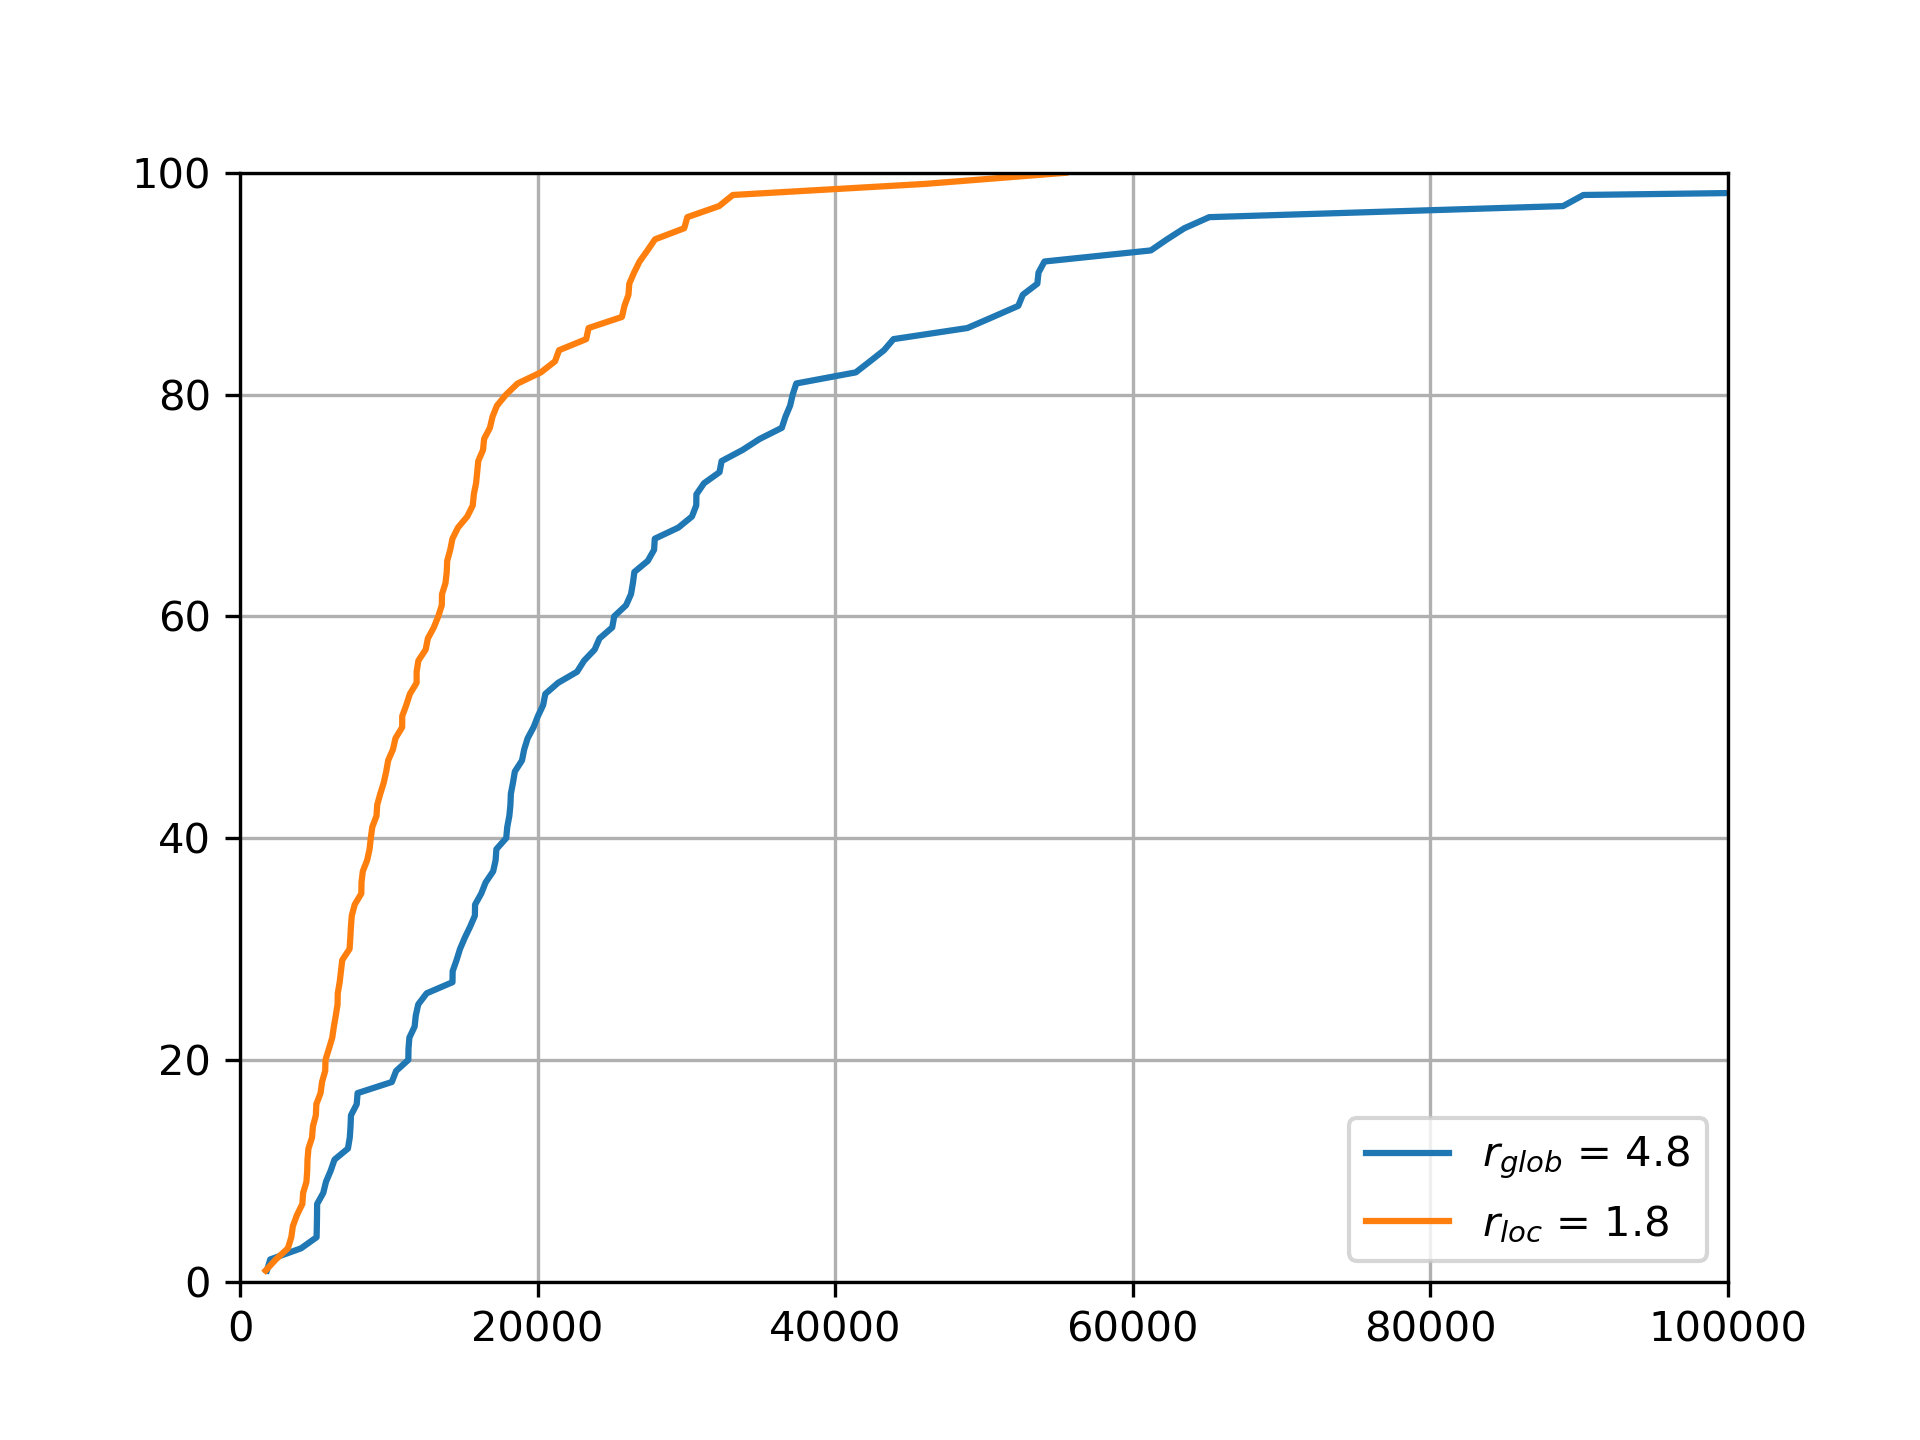
\includegraphics[width=1.0\linewidth]{Operating_characteristic_gklss_4.png} \\ (a)}
\end{minipage}
\hfill
\begin{minipage}{0.5\linewidth}
\center{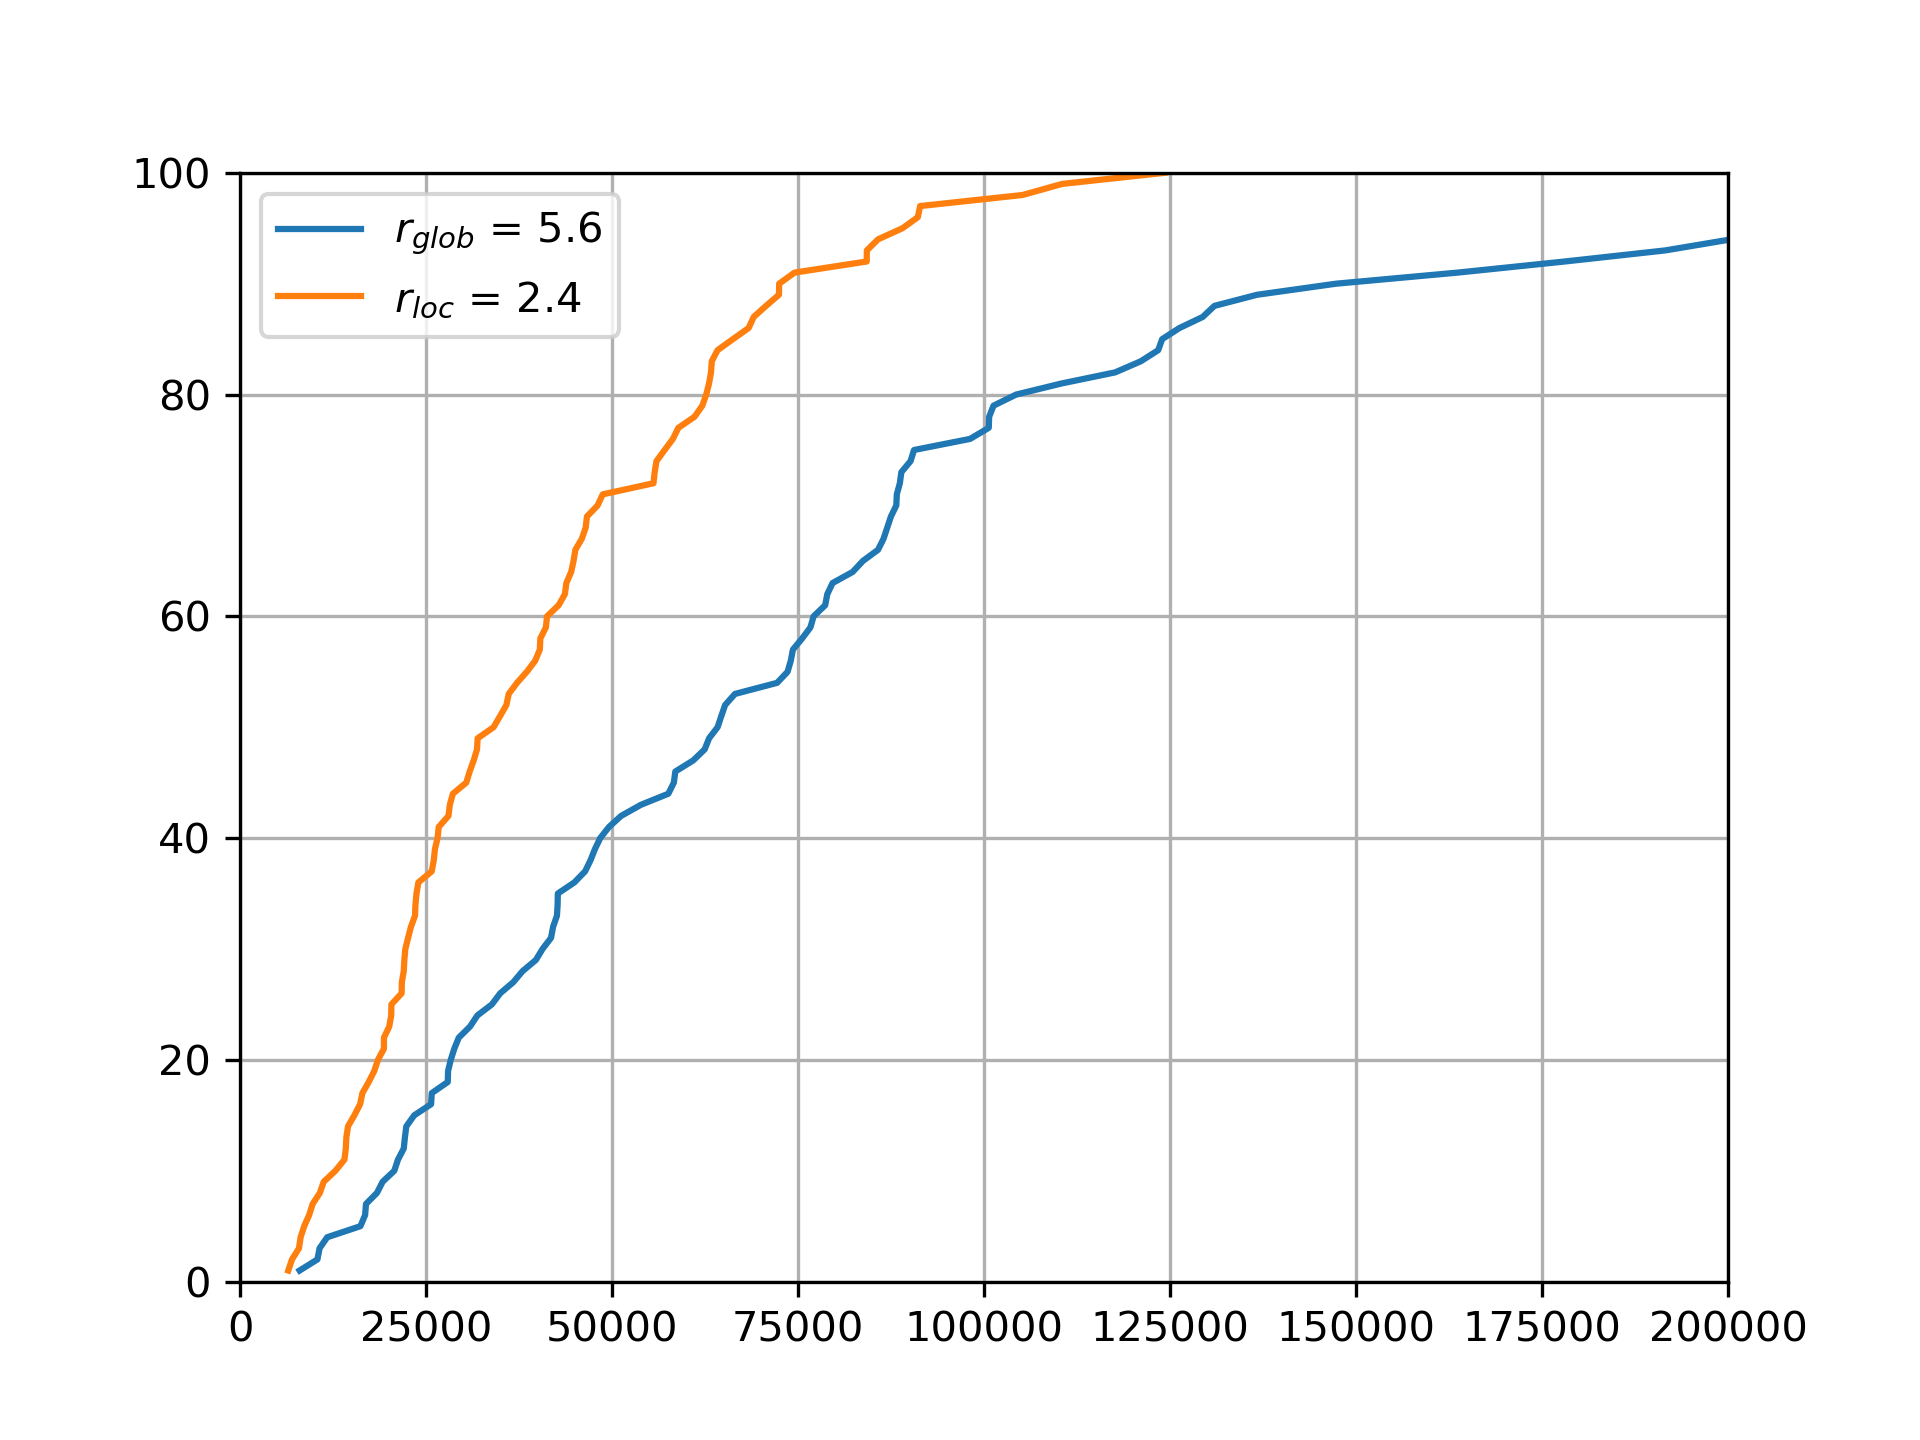
\includegraphics[width=1.0\linewidth]{Operating_characteristic_gklsh_4.png} \\ (b)}
\end{minipage}
\caption{Operational characteristics for GKLS Simple (a) and Hard (b) classes, $N=4$.}
\label{oper4}
\end{figure}

\begin{figure}
\begin{minipage}{0.5\linewidth}
\center{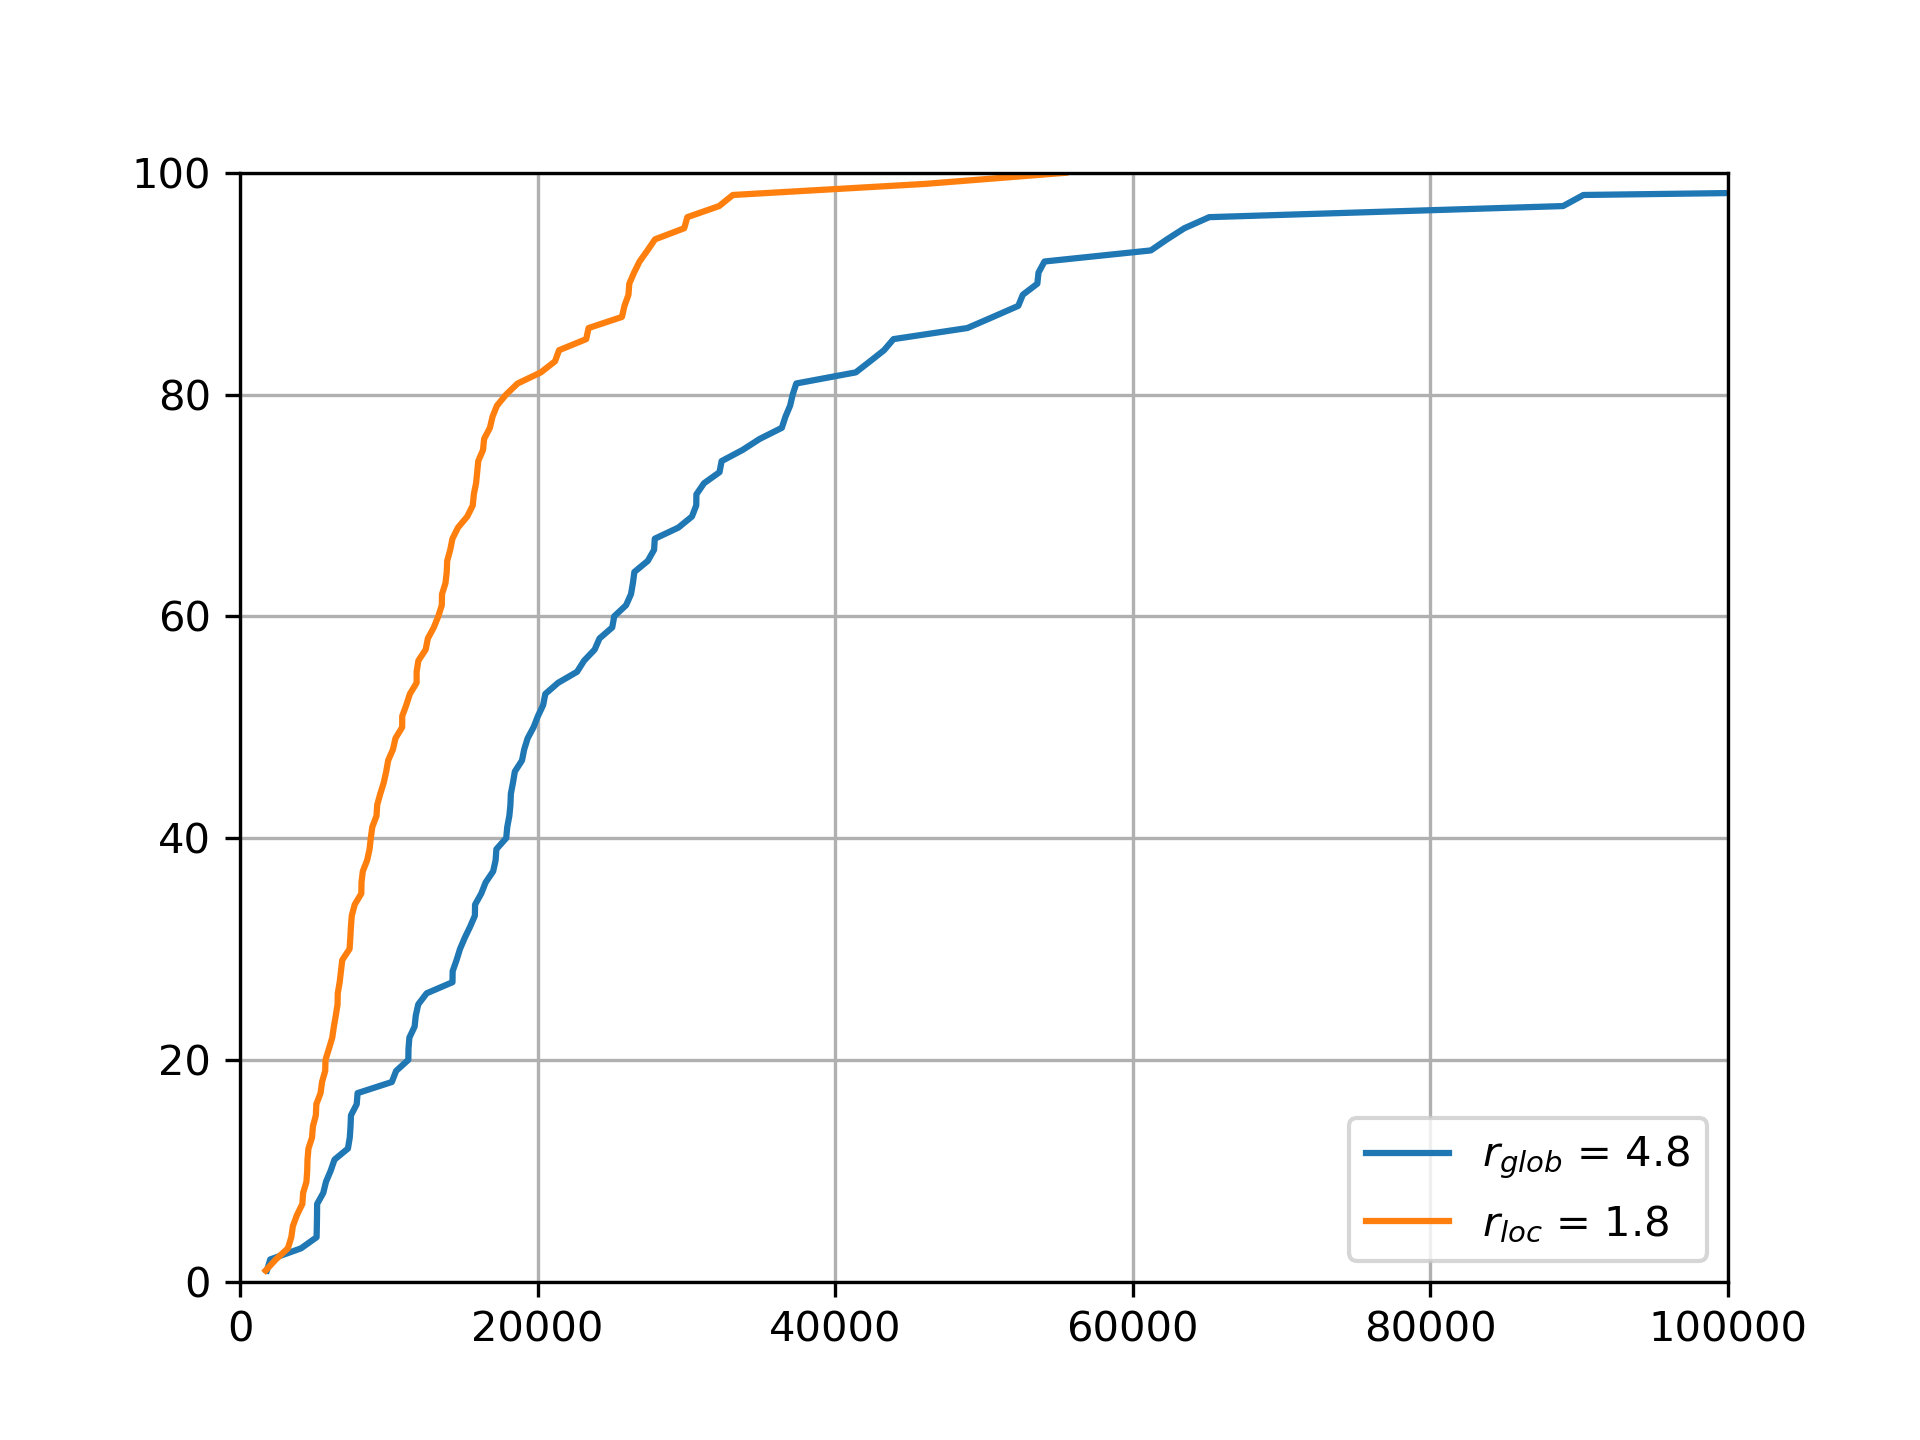
\includegraphics[width=1.0\linewidth]{Operating_characteristic_gklss_4.png} \\ (a)}
\end{minipage}
\hfill
\begin{minipage}{0.5\linewidth}
\center{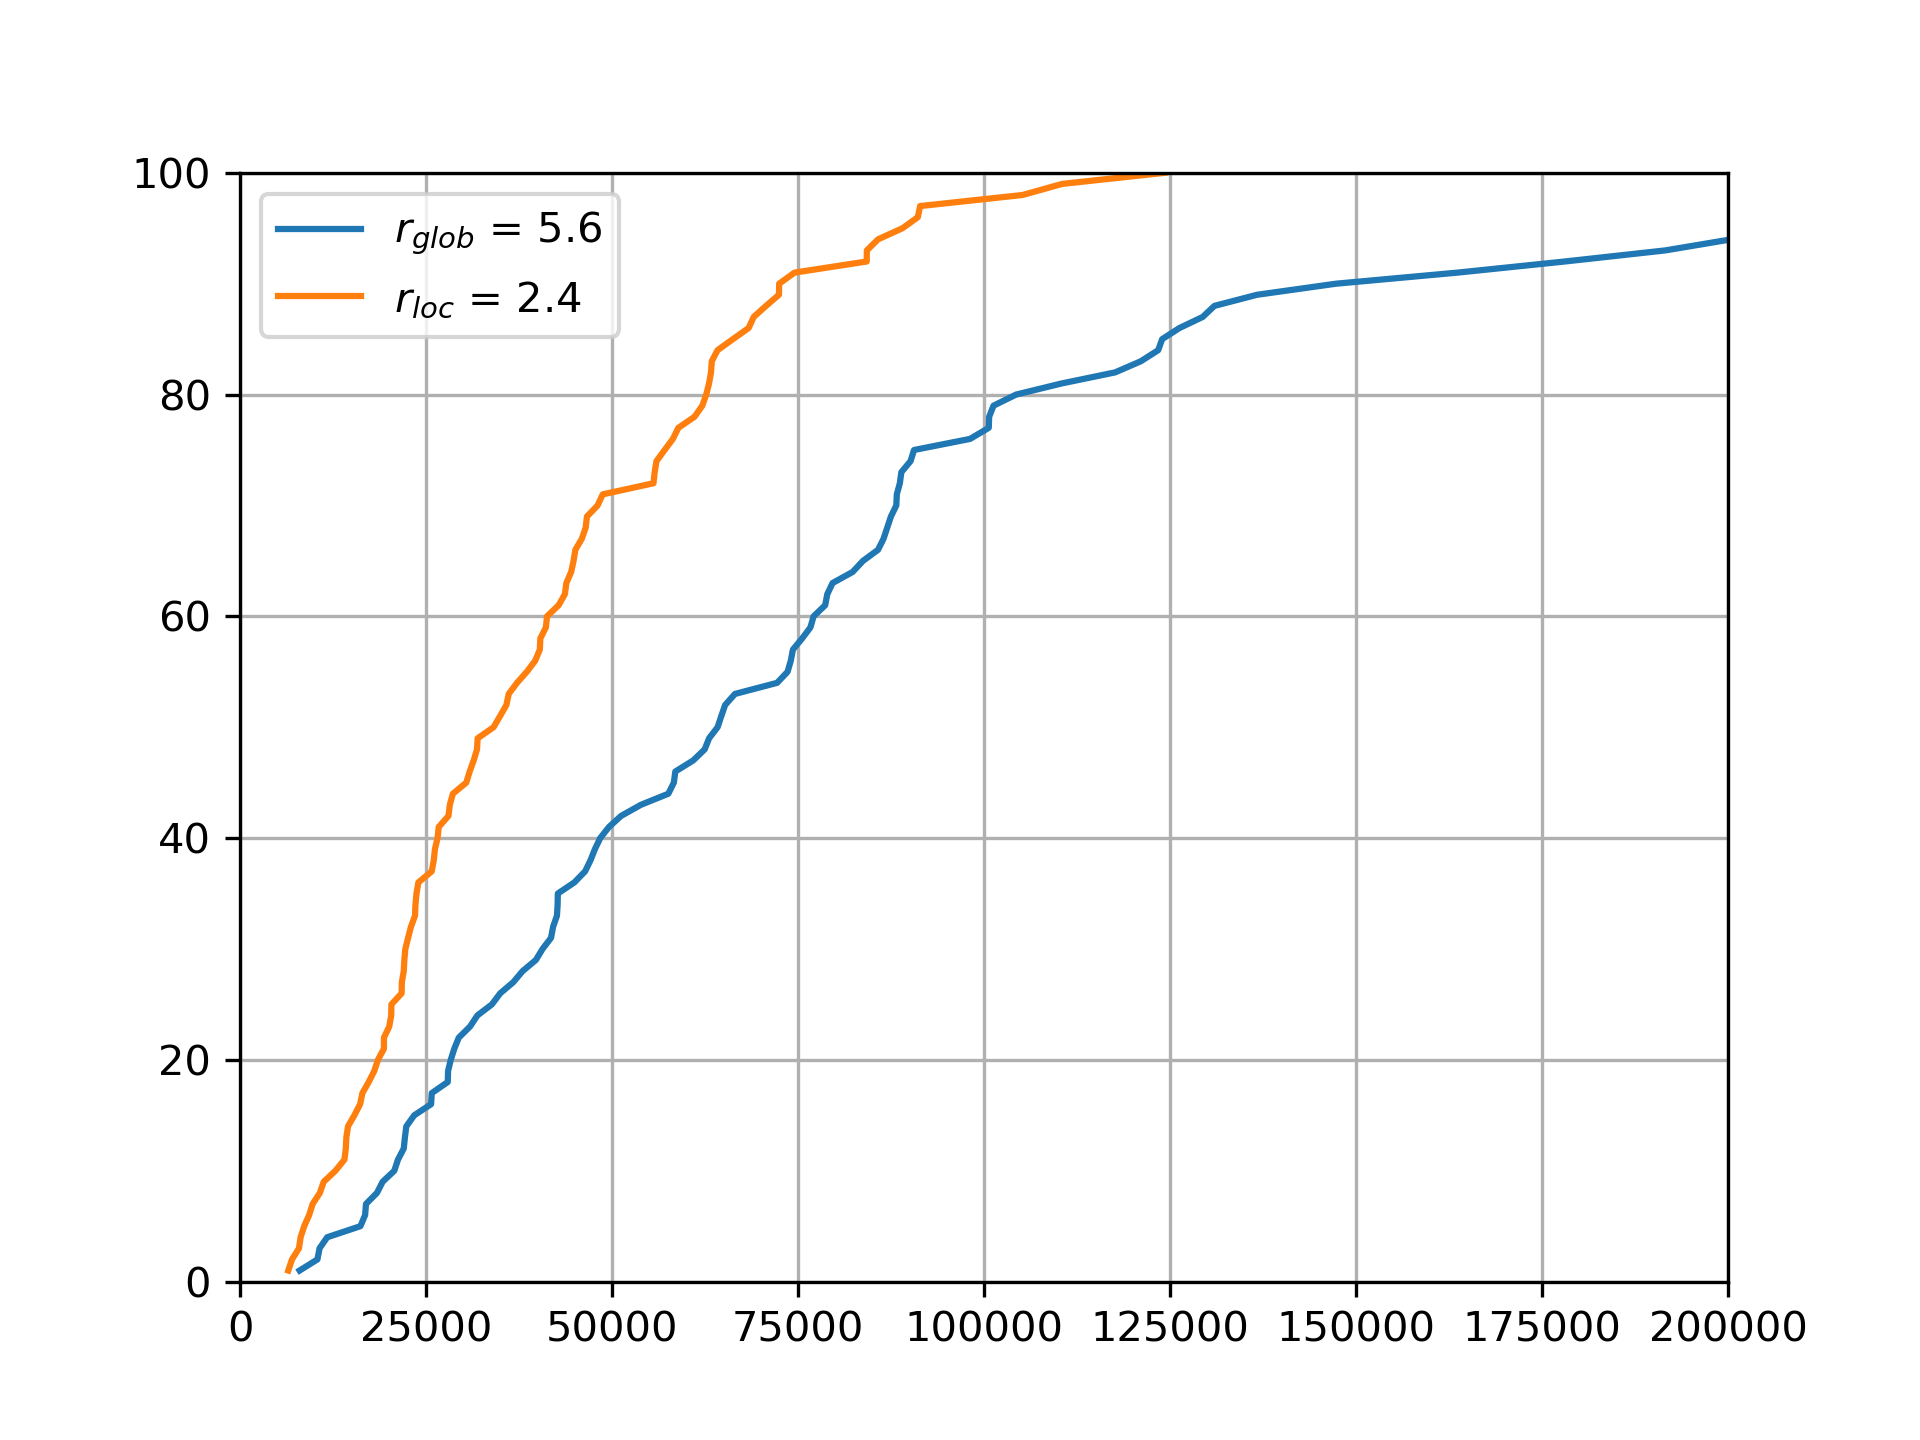
\includegraphics[width=1.0\linewidth]{Operating_characteristic_gklsh_4.png} \\ (b)}
\end{minipage}
\caption{Operational characteristics for GKLS Simple (a) and Hard (b) classes, $N=5$.}
\label{oper5}
\end{figure}


Нижние кривые на обеих фигурах характеризуют GSA, а верхние линии — GSA-DL. Указанное расположение кривых показывает, что алгоритм с двумя оценками константы Липшица обеспечивает в среднем значительно более быстрое решение задач данного класса, чем алгоритм с использованием единственной оценки константы Липшица.

%\section{Conclusion}
%В работе рассматривались задачи глобальной оптимизации, в которых целевая функция удовлетворяет условию Липшица. Был предложен новый способ учета информации о поведения целевой функции в различных подобластях области поиска, основанный на использовании двух оценок константы Липшица, одна из которых значительно больше другой. Сформулированы правила алгоритма, использующего две оценки константы. БОльшая оценка гарантирует сходимость алгоритма к глобальному оптимуму, а одновременное использование меньшей оценки ведет к ускорению сходимости алгоритма. Выбор того, какая из двух оценок будет использоваться в правилах алгоритма, осуществляется адаптивно, в зависимости от поведения функции и фазы поиска.Проведены вычислительные эксперименты, наглядно демонстрирующие эффективность нового алгоритма. При проведении вычислительных экспериментов было решено несколько сотен тестовых многоэкстремальных задач разной размерности.

%
% ---- Bibliography ----
%
% BibTeX users should specify bibliography style 'splncs04'.
% References will then be sorted and formatted in the correct style.

\bibliographystyle{splncs04}
\bibliography{bibliography}

%\begin{thebibliography}{8}
%\end{thebibliography}
\end{document}
